\PassOptionsToPackage{unicode=true}{hyperref} % options for packages loaded elsewhere
\PassOptionsToPackage{hyphens}{url}
%
\documentclass[]{article}
\usepackage{lmodern}
\usepackage{amssymb,amsmath}
\usepackage{ifxetex,ifluatex}
\usepackage{fixltx2e} % provides \textsubscript
\ifnum 0\ifxetex 1\fi\ifluatex 1\fi=0 % if pdftex
  \usepackage[T1]{fontenc}
  \usepackage[utf8]{inputenc}
  \usepackage{textcomp} % provides euro and other symbols
\else % if luatex or xelatex
  \usepackage{unicode-math}
  \defaultfontfeatures{Ligatures=TeX,Scale=MatchLowercase}
\fi
% use upquote if available, for straight quotes in verbatim environments
\IfFileExists{upquote.sty}{\usepackage{upquote}}{}
% use microtype if available
\IfFileExists{microtype.sty}{%
\usepackage[]{microtype}
\UseMicrotypeSet[protrusion]{basicmath} % disable protrusion for tt fonts
}{}
\IfFileExists{parskip.sty}{%
\usepackage{parskip}
}{% else
\setlength{\parindent}{0pt}
\setlength{\parskip}{6pt plus 2pt minus 1pt}
}
\usepackage{hyperref}
\hypersetup{
            pdftitle={Sustainable Development Goals Visual Critique},
            pdfauthor={Eric Scheier \& Matt Ungaro},
            pdfborder={0 0 0},
            breaklinks=true}
\urlstyle{same}  % don't use monospace font for urls
\usepackage[margin=1in]{geometry}
\usepackage{graphicx,grffile}
\makeatletter
\def\maxwidth{\ifdim\Gin@nat@width>\linewidth\linewidth\else\Gin@nat@width\fi}
\def\maxheight{\ifdim\Gin@nat@height>\textheight\textheight\else\Gin@nat@height\fi}
\makeatother
% Scale images if necessary, so that they will not overflow the page
% margins by default, and it is still possible to overwrite the defaults
% using explicit options in \includegraphics[width, height, ...]{}
\setkeys{Gin}{width=\maxwidth,height=\maxheight,keepaspectratio}
\setlength{\emergencystretch}{3em}  % prevent overfull lines
\providecommand{\tightlist}{%
  \setlength{\itemsep}{0pt}\setlength{\parskip}{0pt}}
\setcounter{secnumdepth}{0}
% Redefines (sub)paragraphs to behave more like sections
\ifx\paragraph\undefined\else
\let\oldparagraph\paragraph
\renewcommand{\paragraph}[1]{\oldparagraph{#1}\mbox{}}
\fi
\ifx\subparagraph\undefined\else
\let\oldsubparagraph\subparagraph
\renewcommand{\subparagraph}[1]{\oldsubparagraph{#1}\mbox{}}
\fi

% set default figure placement to htbp
\makeatletter
\def\fps@figure{htbp}
\makeatother


\title{Sustainable Development Goals Visual Critique}
\author{Eric Scheier \& Matt Ungaro}
\date{2/21/2020}

\begin{document}
\maketitle

The 2019 US Cities Sustainable Development Report was developed in
response to rising urbanization in the United States. It is based on the
United Nations' seventeen sustainable development goals that
comprehensively outline what a sustainable, equitable city of the future
will look like. These goals are to be achieved by 2030. The report takes
fifteen of the sustainable goals, assesses various indicators of how
close each metropolitan statistical area is to reaching these goals
through the creation of target values, averages those indicators to
create a goal score, and compares them to the target values.

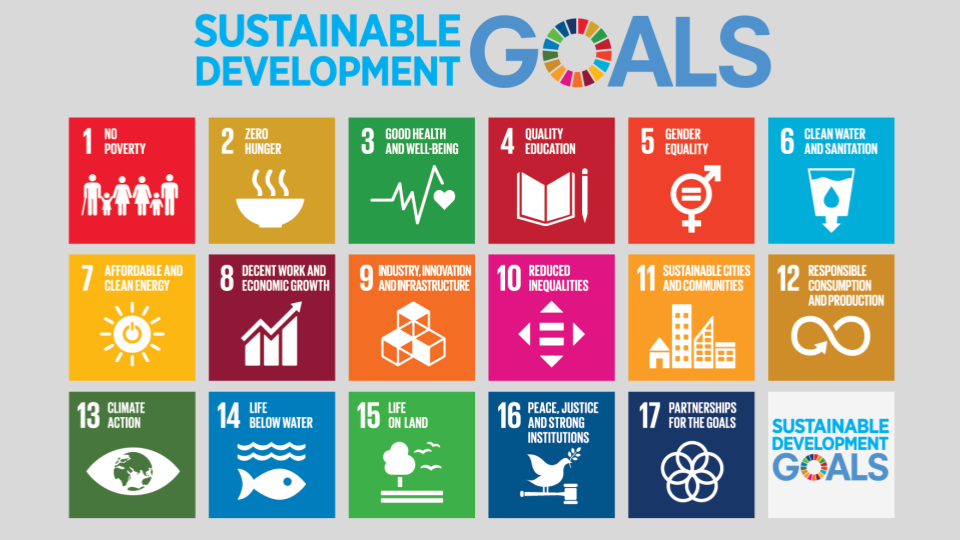
\includegraphics[width=\textwidth,height=\textheight]{sdgs}

For example, goal one is ``no poverty''. There are five indicators of
poverty used to determine how close a metropolitan statistical area is
to exterminating poverty: percentage of population living below the
national poverty line, percentage of children living below twice the
poverty line, percentage of working poor, whether the state, city and
county has a paid sick leave policy, and whether the state, city and
county has a paid family/parental leave policy. These indicators are
averaged and compared to the target value. This is done for the other
fourteen goals with other indicators.

\begin{verbatim}
## # A tibble: 11 x 20
##    rank_sdgIndex maincity score_sdgi score_sdg1 score_sdg2 score_sdg3 score_sdg4
##            <dbl> <chr>         <dbl>      <dbl>      <dbl>      <dbl>      <dbl>
##  1             1 San Fra~         70         84         68         86         61
##  2             2 San Jose         68         87         74         90         65
##  3             3 Washing~         67         84         56         74         65
##  4             4 Seattle          66         83         45         73         57
##  5             5 Madison          66         63         50         72         76
##  6           100 Youngst~         38         22         23         28         40
##  7           101 Bakersf~         38         48         38         36         19
##  8           102 Winston          37         19         18         29         31
##  9           103 Memphis          36         16          7         18         21
## 10           104 Jackson          35         25          9         28         21
## 11           105 Baton R~         30         24         20         25         29
## # ... with 13 more variables: score_sdg5 <dbl>, score_sdg6 <dbl>,
## #   score_sdg7 <dbl>, score_sdg1 <dbl>, score_sdg2 <dbl>, score_sdg3 <dbl>,
## #   score_sdg4 <dbl>, score_sdg5 <dbl>, score_sdg6 <dbl>, score_sdg7 <dbl>,
## #   score_sdg1 <dbl>, score_sdg2 <dbl>, score_sdg3 <dbl>
\end{verbatim}

\begin{verbatim}
## # A tibble: 5 x 13
##   `SDG Alignment` `Indicator name` Description Units   Min   Max `Sort Order`
##   <chr>           <chr>            <chr>       <chr> <dbl> <dbl> <chr>       
## 1 Target 1.2      Living below po~ Percentage~ %         7    30 descending  
## 2 Target 1.1      Childhood pover~ Percentage~ %         3    23 descending  
## 3 Target 1.2      Working poor     Percentage~ %         1    11 descending  
## 4 Target 1.3      Sick leave poli~ Paid sick ~ scor~     0     1 ascending   
## 5 Target 1.3      Family leave po~ Paid famil~ scor~     0     1 ascending   
## # ... with 6 more variables: `Target Value` <dbl>, `To Green` <dbl>, `To
## #   Yellow` <dbl>, `To Orange` <dbl>, `Worst Value` <dbl>, `Threshold
## #   Rationale` <chr>
\end{verbatim}

The main visualization of the report was Figure 2: Dashboard. It
portrays the relative statuses of US cities toward meeting the UN
Sustainable Development Goals. It is successful in that it tells an
intuitive story that can be comprehended by anyone. It is
reaction-inducing. It also summarizes a variety of data types in a way
that can be understood. Unfortunately, it has a story that could also be
misinterpreted by individuals. It must be viewed over two pages to be
understood because it has a limited color scale that only has a key on
the second page. It does not cover every sustainable development goal.
Finally, the index scores are not completely clear.

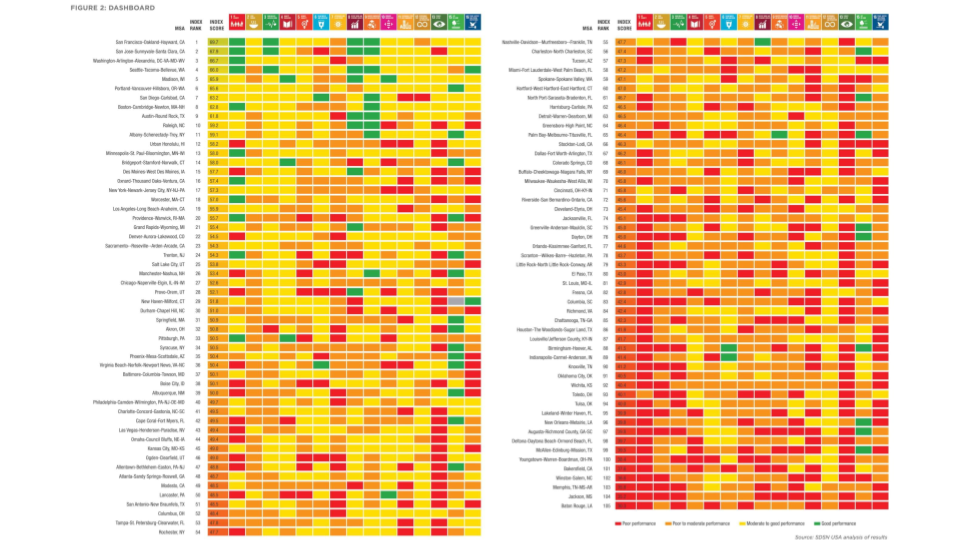
\includegraphics[width=\textwidth,height=\textheight]{sdg_dashboard}

Because of the choice of the colors, we believe that the objective of
this visualization was to elicit an emotional reaction. Based merely on
these images, we do not know how bad red is and how good green is,
beyond what is shown at the bottom of page 13. Red means poor
performance, orange means poor to moderate performance, yellow means
moderate to good, and green means good performance. That does not
explain what ``poor'' and ``good'' mean in this context. Only later is
it mentioned that green blocks mean that a metropolitan area has already
met the 2030 goals. This tells us that the goal of this chart was not to
show technicalities but to elicit an emotional reaction. They could
influence a reader's feelings about the United States' progress.
Policymakers could see the colors and feel motivated to focus on certain
blocks and create change. However, these colors could also elicit
negative reactions. Individuals might feel bad or apathetic; if the
United States' is so behind on the SDGs, what is the point of trying?
With so much red and orange, policymakers might feel angry or even
attacked and choose to disregard the SDGs. The visualization of these
goals helps to tell the story that the authors are conveying, but it
also generalizes the story.

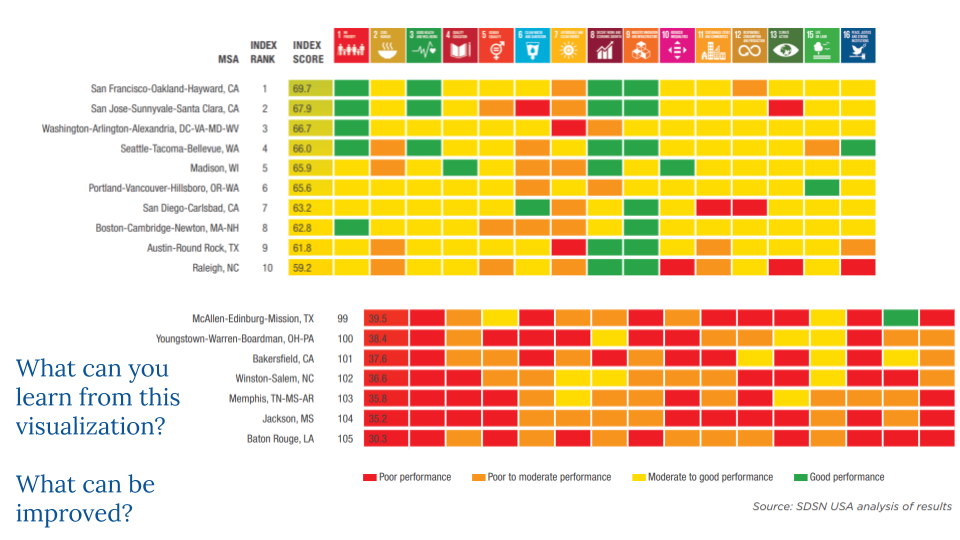
\includegraphics[width=\textwidth,height=\textheight]{chart_slice}

The story that the authors are trying to tell with this figure is that
the United States is failing to achieve many of the Sustainable
Development Goals. Every city needs to take much larger steps to reach
these goals by 2030. However, looking at the underlying data, while this
probably is a good interpretation, there are potentially other ones. For
example, the authors used 57 indicators to convey data for the goals.
However, the authors also acknowledge that there are potentially
hundreds of other indicators that they could have chosen to draw from to
create this figure. Perhaps including those other indicators may have
led to large changes in the visualization.

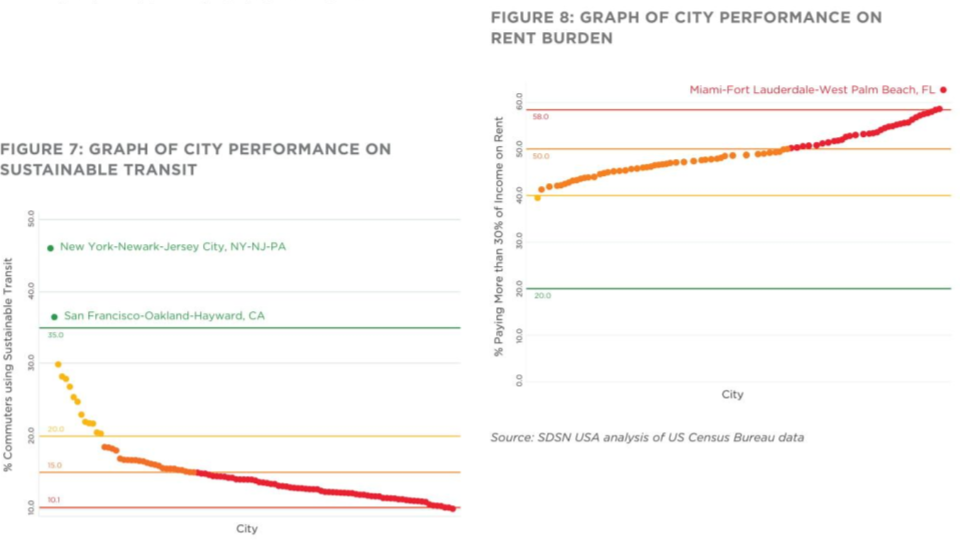
\includegraphics[width=\textwidth,height=\textheight]{cutaway}

By choosing to show data using four colors and index scores, Figure 2's
authors obscured the complexity of the data that they are pulling from.
Some of the data is binary; for example, the existence of a metropolitan
government's paid sick leave policy warrants a 1 and if lacking,
warrants a 0. That translates to a score of 100 or 0. Other data, like
population with health insurance, is based on percentages, while LGBTQ
inclusivity of laws, policies, and services is based on an 0-100 index.
These four colors do not capture the diversity of the various
measurements. Additionally, the choices of colors make it potentially
appear that the United States is doing worse than it is. Yellow means
moderate to good, but in this chart, surrounded by red and orange,
yellow tends to be ignored by the eye or placed into a negative
category, even though it might mean that a city is very close to meeting
its goal in one of the yellow blocks. Finally, there is a weighting
mechanism underlying the data that is not present in the figure. This
can lead to peculiarities. For example, while Honolulu has a higher
score than Minneapolis, Minneapolis has more green and yellow blocks
than Honolulu. Honolulu has more red and orange ones. This could lead to
even greater confusion, particularly for individuals comparing
metropolitan areas.


\includegraphics[width=\textwidth,height=\textheight]{min_hon}

There are a few better choices for this graphic. One, the graphic should
have goals that are easier to read -- practically speaking, larger text
could be appropriate. The pictures are not necessarily easy to
understand. Perhaps yellow could have been split into yellow and light
green, to show if a city is actually close to achieving its goals and
encouraging readers of this graphic. While this might complicate the
graphic, the writers could have subdued the colors and placed numbers
over the blocks to show how each metropolitan area scored on each goal.
The average of the indicators could be overlaid on the blocks. This
could elicit a less emotional reaction and give policymakers clarity on
how their cities compare to other cities. Finally, the graphic could be
discarded altogether, and a bar chart for each city showing the city
average for each goal could be created, with reference to the various
indicators that were averaged to create these.

\hypertarget{reference}{%
\section{Reference}\label{reference}}

Lynch, A., LoPresti, A., Fox, C. (2019): The 2019 US Cities Sustainable
Development Report. New York: Sustainable Development Solutions Network
(SDSN).

\end{document}
